\documentclass{article}
\usepackage{tikz}
\usetikzlibrary{positioning}

\begin{document}
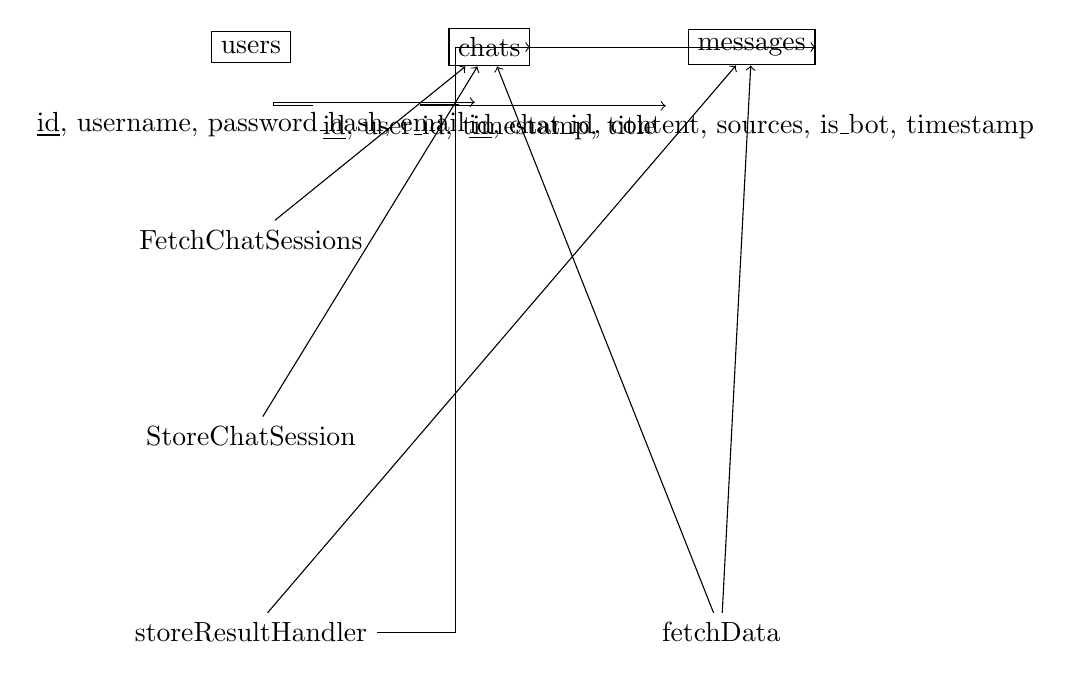
\begin{tikzpicture}[node distance=2cm]
  % Users table
  \node[rectangle, draw] (users) {users};
  \node[below=0.5cm of users] (users_cols) {\underline{id}, username, password\_hash, email};

  % Chats table
  \node[rectangle, draw, right=of users] (chats) {chats};
  \node[below=0.5cm of chats] (chats_cols) {\underline{id}, user\_id, timestamp, title};
  \draw[->] (chats_cols.north west) -- ++(-0.5cm,0) |- (users_cols.north east);

  % Messages table
  \node[rectangle, draw, right=of chats] (messages) {messages};
  \node[below=0.5cm of messages] (messages_cols) {\underline{id}, chat\_id, content, sources, is\_bot, timestamp};
  \draw[->] (messages_cols.north west) -- ++(-0.5cm,0) |- (chats_cols.north east);

  % Interactions
  \node[below=of users] (fetch) {FetchChatSessions};
  \node[below=of fetch] (store1) {StoreChatSession};
  \node[below=of store1] (store2) {storeResultHandler};
  \node[right=of store2, xshift=1.5cm] (fetchData) {fetchData};

  \draw[->] (fetch) -- (chats);
  \draw[->] (store1) -- (chats);
  \draw[->] (store2) -- (messages);
  \draw[->] (store2.east) -- ++(1cm,0) |- (chats.east);
  \draw[->] (store2.east) -- ++(1cm,0) |- (messages.east);
  \draw[->] (fetchData) -- (chats);
  \draw[->] (fetchData) -- (messages);
\end{tikzpicture}
\end{document}
	
